\mode<presentation>
{
  \usetheme{CambridgeUS}
  \usecolortheme{whale}
  \usecolortheme{lily}

  \setbeamercovered{transparent}
  \usefonttheme[onlymath]{serif}
}

\title[\MotorControlShortName] % (optional, use only with long paper titles)
{\course: \MotorControlName\license}

\subtitle
{Lecture \MotorControlNumber} % (optional)



\begin{document}

\begin{frame}
  \titlepage
\end{frame}

\mode<article>{
\maketitle
\tableofcontents
}

%\mode<presentation>{
%\begin{frame}{Outline}
%  \tableofcontents
%  % You might wish to add the option [pausesections]
%\end{frame}}

\section{Pre-requisite Material}
This lecture assumes that the reader is familiar with the following material:
\begin{itemize}
	\item Lecture \PIDControlDesignNumber:~\PIDControlDesignName
	\item Lecture \MotorModelingNumber:~\MotorModelingName
\end{itemize}


\section{Feedback Control for DC Motors
\label{sec:MotorControl}}

As mentioned in Lecture \MotorModelingNumber:~\MotorModelingName, DC motors are used in many applications. Although the process for modeling the DC motor may seem a little more complicated than for other types of systems we have studied, the control design process and verification is essentially the same. We will likely still have specifications in terms of the steady state response (e.g., reference tracking, disturbance rejection) and transient response (e.g., rise time, settling time, and percent overshoot in response to a step input) that will impact both our choice of controller structure and the gain values $K_P$, $K_I$, and $K_D$ that we select. 

Starting with the DC motor plant system with arbitrary load:
\begin{frame}{DC motor block diagram with arbitrary load}
\begin{center}
	\input{figures/motorblockdiagram2.tex}
\end{center}
\end{frame}
\noindent we first emphasize that this system with input $V_a(s)$ and output $\theta(s)$ is the \textit{open loop plant}, i.e., the $G(s)$ that is a single block in our standard closed-loop feedback control system, as is shown in the next two block diagrams. 

%\begin{frame}{\textcolor{red}{Frame Content for Presentation File}}
%\begin{center}
%\mode<article>{\includegraphics[width=4.5in]{figures/emptyfig.png}
}
%\mode<presentation>{\resizebox{3in}{!}{\includegraphics[width=4.5in]{figures/emptyfig.png}
}}
%\end{center}
%\end{frame}


\begin{frame}{DC motor block diagram is the open loop plant}
\begin{center}
\mode<article>{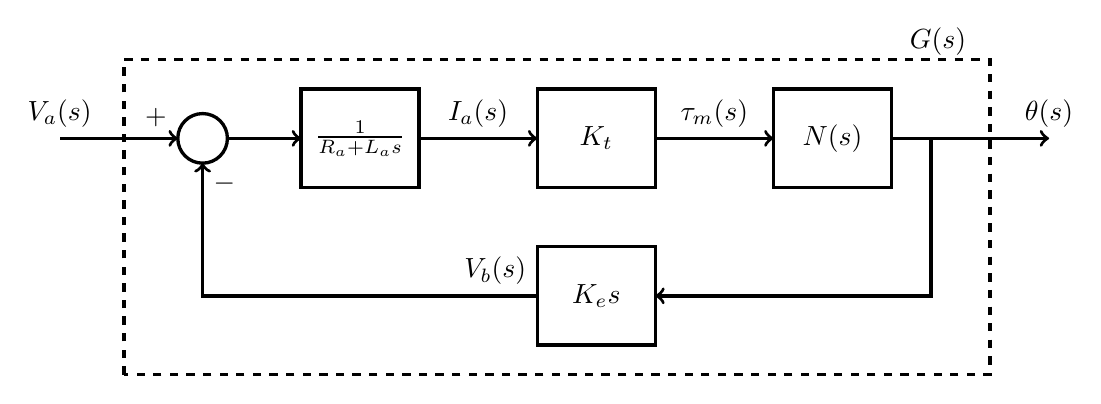
\begin{tikzpicture}[inner sep=0pt,outer sep=0pt,very thick,
sysblock/.style={draw,rectangle,inner sep=2pt,minimum width=1.5cm,minimum height=1.25cm,very thick}]

\draw (0,0) node[draw,circle] (sum) {$\rule{0pt}{18pt}$};
\draw (2,0) node[sysblock] (a) {$\frac{1}{R_{a} + L_{a}s}$};
\draw (5,0) node[sysblock] (b) {$K_{t}$};
\draw (8,0) node[sysblock] (c) {$N(s)$};
\draw (5,-2) node[sysblock] (d) {$K_{e}s$};

\draw[<-] (sum.180) node[above left=4pt] {$+$} -- ++(-1.5,0) node[above=4pt] {$V_{a}(s)$};
\draw[->] (sum.0) -- (a.180);
\draw[->] (a.0) -- node[pos=.5,above=4pt] {$I_{a}(s)$} (b.180);
\draw[->] (b.0) -- node[pos=.5,above=4pt] {$\tau_{m}(s)$} (c.180);
\draw[->] (c.0) -- ++(2,0) node[above=4pt] {$\theta(s)$} node[above left=30pt] {$G(s)$};
\draw[->] (c.0) -- ++(.5,0) |- (d.0);
\draw[->] (d.180) node[above left=4pt] {$V_{b}(s)$} -| (sum.-90) node[below right=4pt] {$-$};

\draw [dashed] (sum) ++(-1,-3) rectangle ++(11,4);

\end{tikzpicture}}
\mode<presentation>{\resizebox{4.5in}{!}{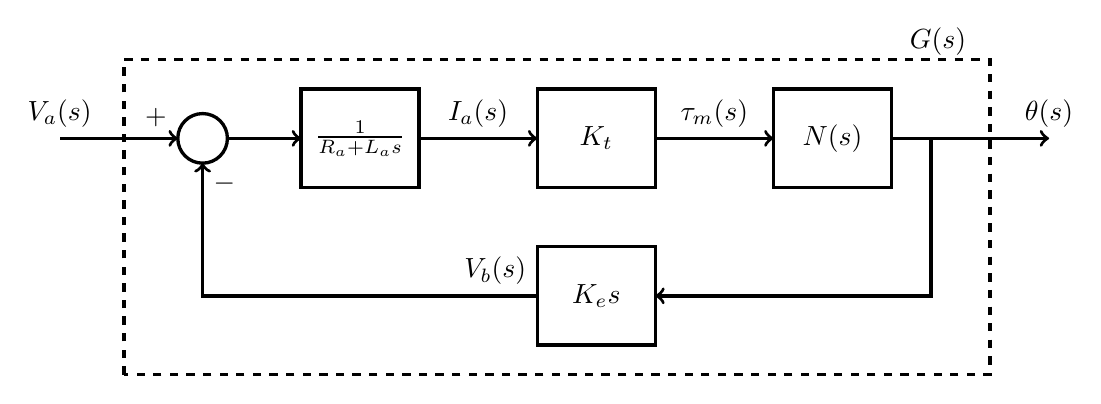
\begin{tikzpicture}[inner sep=0pt,outer sep=0pt,very thick,
sysblock/.style={draw,rectangle,inner sep=2pt,minimum width=1.5cm,minimum height=1.25cm,very thick}]

\draw (0,0) node[draw,circle] (sum) {$\rule{0pt}{18pt}$};
\draw (2,0) node[sysblock] (a) {$\frac{1}{R_{a} + L_{a}s}$};
\draw (5,0) node[sysblock] (b) {$K_{t}$};
\draw (8,0) node[sysblock] (c) {$N(s)$};
\draw (5,-2) node[sysblock] (d) {$K_{e}s$};

\draw[<-] (sum.180) node[above left=4pt] {$+$} -- ++(-1.5,0) node[above=4pt] {$V_{a}(s)$};
\draw[->] (sum.0) -- (a.180);
\draw[->] (a.0) -- node[pos=.5,above=4pt] {$I_{a}(s)$} (b.180);
\draw[->] (b.0) -- node[pos=.5,above=4pt] {$\tau_{m}(s)$} (c.180);
\draw[->] (c.0) -- ++(2,0) node[above=4pt] {$\theta(s)$} node[above left=30pt] {$G(s)$};
\draw[->] (c.0) -- ++(.5,0) |- (d.0);
\draw[->] (d.180) node[above left=4pt] {$V_{b}(s)$} -| (sum.-90) node[below right=4pt] {$-$};

\draw [dashed] (sum) ++(-1,-3) rectangle ++(11,4);

\end{tikzpicture}}}
\end{center}
\end{frame}

\begin{frame}{Feedback control of DC motor with plant shown}
\begin{center}
\mode<article>{\begin{tikzpicture}[inner sep=0pt,outer sep=0pt,very thick,
sysblock/.style={draw,rectangle,inner sep=2pt,minimum width=1.5cm,minimum height=1.25cm,very thick}]

\draw (0,0) node[draw,circle] (sum) {$\rule{0pt}{36pt}$};
\draw (2.5,0) node[sysblock] (z) {Controller $C(s)$};
\draw (8,0) node[sysblock] (y) {\resizebox{2.5in}{!}{\input{figures/motorblockdiagram2b.tex}}};
\draw (12,0) node (x) {};

\draw[<-] (sum.180) node[above left=4pt] {$+$} -- ++(-1.5,0) node[above=4pt] {$R(s)$};
\draw[->] (sum.0) -- (z.180);
\draw[->] (z.0) -- node[pos=.5,above=4pt] {$V_{a}(s)$} (y.180);
\draw[->] (y.0) -- ++(1,0) node[above=4pt] {$\theta(s)$};
\draw[->] (x.-90) -- ++(0,-2) -| (sum.-90) node[below right=4pt] {$-$};


\end{tikzpicture}}
\mode<presentation>{\resizebox{4.5in}{!}{\begin{tikzpicture}[inner sep=0pt,outer sep=0pt,very thick,
sysblock/.style={draw,rectangle,inner sep=2pt,minimum width=1.5cm,minimum height=1.25cm,very thick}]

\draw (0,0) node[draw,circle] (sum) {$\rule{0pt}{36pt}$};
\draw (2.5,0) node[sysblock] (z) {Controller $C(s)$};
\draw (8,0) node[sysblock] (y) {\resizebox{2.5in}{!}{\input{figures/motorblockdiagram2b.tex}}};
\draw (12,0) node (x) {};

\draw[<-] (sum.180) node[above left=4pt] {$+$} -- ++(-1.5,0) node[above=4pt] {$R(s)$};
\draw[->] (sum.0) -- (z.180);
\draw[->] (z.0) -- node[pos=.5,above=4pt] {$V_{a}(s)$} (y.180);
\draw[->] (y.0) -- ++(1,0) node[above=4pt] {$\theta(s)$};
\draw[->] (x.-90) -- ++(0,-2) -| (sum.-90) node[below right=4pt] {$-$};


\end{tikzpicture}}}
\end{center}
\end{frame}


\begin{frame}{DC Motor Control Video Example}
Consider the DC motor control problem shown in the video  \url{https://www.youtube.com/watch?v=dTGITLnYAY0}. %More info on the physical connections/hardware (encoder, arduino, ) and needed software. Maybe too much software/code? Could skip some and then re-start at the block diagram around 4:24.
\end{frame}

While watching the video, please respond to the following prompts:

\begin{frame}{DC Motor Control Prompts}
\begin{itemize}
	\item What hardware is needed? Consider plant (DC motor), sensor, actuator and controller. %microcontroller, DC motor with encoder, and motor driver
%	\item<2-> What software is needed for the motor position measurement (from the encoder)? Does the position measurement algorithm increment or decrement the position value from a stored value in a similar manner to a discrete-time integral?
	\item<2-> What two physical components are considered as part of the ``plant'' in the video? %motor and motor driver
	\item<3-> What is the reference input signal called in the video? %target position
	\item<4-> What kind of controller is used in the video? %PID
	\item<5-> How are the integral and derivative terms estimated in this discrete-time control algorithm? %finite difference equation
	\item<6-> What is the performance of the feedback controller at the first test? Consider both steady-state and transient (rise time, settling time, and percent overshoot) response. %percent overshoot is present and not desired
	\item<7-> What control term is tuned to solve the problem identified in the previous step? %derivative
	\item<8-> What reference input signals are used? %step, sinusoid
	\item<9-> What types of disturbances are expected to impact the DC motor system? %not specified in the video
\end{itemize}
\end{frame}
Note that the video shows some Arduino code that goes beyond what we will learn specifically in \course~but that could be helpful if you have a control-related project in another class. 




\section{DC Motor Position Control Example}

%Note to self: example is from the old PID control lecture.
\begin{example}\label{ex:examplePD} Let's look at the problem of designing a controller so that a motor can accurately position a rotational load. In other words, we want the output signal $\theta$ to track a desired reference $r$ with parameters and specifications to be provided below. 
	\begin{frame}
	\begin{center}
		\input{figures/motordiagram2.tex}
		\mode<presentation>{
			$R_{a}=1$, $L_{a}=0$, $J=1$, $b=2$, $K_{e}=K_{t}=1$
			\begin{itemize}
				\item rise time, $t_{r}=.1$ s
				\item overshoot, $\% OS=10\%$.
			\end{itemize}
		}
	\end{center}
\end{frame}
The system parameters are: $R_{a}=1$, $L_{a}=0$, $J=1$, $b=2$, $K_{e}=K_{t}=1$. We want to design a controller so that the orientation $\theta$ will follow a step reference with specifications:
\begin{itemize}
	\item rise time, $t_{r}=.1$ s
	\item overshoot, $\% OS=10\%$.
\end{itemize}
By comparison of this example to the one in Lecture \MotorModelingNumber:~\MotorModelingName, we can see that the (open loop) transfer function $\theta(s)/V_{a}(s)$ is
\[
\frac{\theta(s)}{V_{a}(s)} = \frac{K_{t}}{s((Js+b)(R_{a}+L_{a}s) +K_{t}K_{e})} = \frac{1}{s((s+2)+1)} = \frac{1}{s^{2}+3s}
\]	
Notice that both of the specifications are related to transient response, so it might be a good idea to try a $PD$ control structure first. Let's use the ``Physically-derived'' system configuration (Lecture~\PDControlTransientNumber) for this example, in which case the closed-loop system block diagram looks like the following:
\begin{frame}
\begin{center}
	\input{figures/PDexampleblockdiagram.tex}
	
	\mode<presentation>{
		\[
		\frac{\theta(s)}{R(s)} = \frac{K_{p}}{s^{2}+(3+K_{d})s+K_{p}}
		\]
		$\omega_{n}^{2} = K_{p}$, $2\zeta\omega_{n} = 3+K_{d}$ and $K=1$
	}
\end{center}
\end{frame}
\end{example}
Because the system is second order with no zeros, it is possible to choose the gains $K_{p}$ and $K_{d}$ directly from the closed loop transfer function. In this case, the closed loop transfer function from the reference command is
\[
\frac{\theta(s)}{R(s)} = \frac{K_{p}}{s^{2}+(3+K_{d})s+K_{p}}
\]
This looks like our canonical second order system
\[
G(s) = K\frac{\omega_{n}^{2}}{s^{2}+2\zeta\omega_{n}s+\omega_{n}^{2}}
\]
with $\omega_{n}^{2} = K_{p}$, $2\zeta\omega_{n} = 3+K_{d}$ and $K=1$.

To choose $K_{p}$ and $K_{d}$, we find a set of complex conjugate poles that will meet our specifications. Remember that we have already parameterized our specifications in terms of $\zeta$ and $\omega_{n}$:
\begin{frame}
\begin{itemize}
\item $\tr = \treqtwo = .1$ implies $\omega_{n} = 22$
\item $\OS = $10\% implies $\zeta = \frac{-\ln\left(\frac{10\%}{100 \%}\right)}{\sqrt{\ln\left(\frac{10\%}{100 \%}\right)^2+\pi^2}}=.59$
\end{itemize} 
\mode<article>{Thus}
\begin{align*}
K_{p}& = \omega_{n}^{2} =  22^2 = 484 \\
K_{d}& = 2\zeta\omega_{n} - 3 = 2(.59)(22) - 3 =  22.96
\end{align*}
\end{frame}





\section{Application Example}

Consider the DC motor control example shown in the video \url{https://www.youtube.com/watch?v=ojuAATNIfNE}. Respond to these prompts for the example in this video, which are similar to those in Section~\ref{sec:MotorControl}. 

\begin{itemize}
	\item What hardware is needed? Consider plant (DC motor), sensor, actuator and controller. \\ \textit{A Quanser DC motor is shown but not specified.}	
	\item What kind of model validation is done in the video prior to developing a feedback controller? \\ \textit{The video shows a ``bump test'', which entails changing the open-loop plant's input voltage $v_a(t)$ in a series of steps and adjusting the model parameters to better match the experimental results. We will do something similar in the upcoming Lecture~\SystemIdentificationNumber:~\SystemIdentificationName.}
	\item What kind of controller is used in the video? \\ \textit{PID control}
	\item What is the performance of the feedback controller at the first test? Consider both steady-state and transient (rise time, settling time, and percent overshoot) response. \\ \textit{In the speed control experiment, we see high percent overshoot and a long settling time. In the position control experiment}
	\item What control term is tuned to solve the problem identified in the previous step? \\ \textit{In the speed control experiment, proportional and integral gains. In the position control experiment, proportional and derivative gains.}
	\item What reference input signals are used? \\ \textit{In both experiments, the reference signals are steps (i.e., ``stepwise constant'' changes in desired speed or desired position).}
	\item What types of disturbances are expected to impact the DC motor system? \\ \textit{step}
\end{itemize}


\section{Lecture Highlights}
The primary takeaways from this article include
\begin{enumerate}
\setlength{\itemsep}{5pt}
\setlength{\parskip}{0pt}
\setlength{\parsep}{0pt}
\item A common point of confusion with DC motors is that the feedback path inherent in the DC motor path is a feedback controller, but it is not. 
\item Once the plant model $G(s)$ has been obtained, controlling a DC motor requires the same process of evaluating specifications, selecting control parameters, and verifying performance as the design of controllers for other types of systems that we have done in this class.
\end{enumerate}

%\section{Quiz Yourself}
%
%\subsection{Questions}
%\begin{enumerate}
%\setlength{\itemsep}{5pt}
%\setlength{\parskip}{0pt}
%\setlength{\parsep}{0pt}
%\item \input{quizfigures/quizyourself1.tex} 
%\end{enumerate}
%
%\subsection{Solutions}
%
%\begin{enumerate}
%\setlength{\itemsep}{5pt}
%\setlength{\parskip}{0pt}
%\setlength{\parsep}{0pt}
%\item \rule{0pt}{12pt}\\  % use this \rule command to correctly align solutions given as images
%\begin{center}
%\includegraphics[width=4.5in]{quizfigures/emptyfig.png}
%\end{center}\newpage
%\end{enumerate}



\end{document}


